% !TeX document-id = {9ccc6fb7-c5f4-4308-9c17-4c226ad62230}
%%%%%%
%
% $Autor:  $
% $Datum: 2023-01-31 11:59:00Z $
% $Version: 1.0.0 $
%
%
% !TeX encoding = utf8
% !TeX root = Rename
% !TeX TXS-program:bibliography = txs:///biber
%
%%%%%%


\chapter{Domain Knowledge}\label{DomainKnowledge}

The main scope of our project is to incorporate the ESP32 Cam device to convert the analog readings in the water and electricity meter into a digital one. The ESP32 cam will detect the last numerical digit from the electricity meter and convert it into a digital one.

\section{TinyML}

TinyML is a field of study which lies in the Machine Learning, Deep Learning and Embedded Systems which explores the various types of models that can run on relatively compact and energy efficient devices such as microcontrollers.\cite{Arun:2020} The TinyML is capable of running both machine learning as well as deep learning models in resource constrained devices which are of small size and consumes low power of few milliwatt or lesser. Due to the limited memory available on these devices, large machine learning models are optimised and reduced in size.

The TinyML provides a number of advantages over the traditional machine learning like low-latency, low bandwidth and low power consumption while still having the functionality to be transformed into a large machine learning model. It also eliminates the privacy limitations of traditional Machine Learning as the model runs on edge devices which does not store your data in any servers.\cite{Arun:2020}

\section{TensorFlow/TensorFlow Lite/TensorFlow Micro}
TensorFlow is an open-source software library which was developed by Google to build and train machine learning models with deep neural networks. TensorFlow Lite is a lighter version of the TensorFlow.
TensorFlow Lite is also an open-source deep learning framework which is specifically designed for on-device computing in edge devices. TensorFlow Lite enables the developers to run their trained models on edge devices, computers and mobiles. TensorFlow Lite provides the ability to perform predictions on an already trained model.\cite{Boesch:2022}

\begin{figure}  
	\begin{center}
		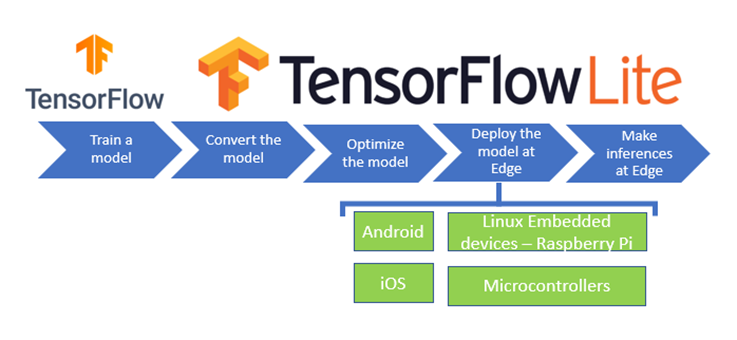
\includegraphics[width=12cm]{ESP32/TFLworkflow}
		\caption{Tensor Flow Lite Workflow} 
		\label{fig:Visual Studio Code Download Options}
		\footnotesize \textbf{Reference:} \cite{Khandelwal:2020}
	\end{center}
\end{figure}

TensorFlow Lite Microcontrollers (TFLM) is designed to run machine learning models and deep learning models on microcontrollers with only a few kilobytes of memory. TFLM tackles both the efficiency requirements imposed by embedded-system resource constrains as well as the fragmentation challenges and makes cross-platform interoperability possible. The TFLM framework adopts a unique interpreter-based approach that provides flexibility while overcoming the forementioned challenges.\cite{Robert:2021}

%%%%%%%%%%%%%%%%%%%%%%%%%%%%%%%
\section{Algorithm: Convolutional Neural Network}

Convolutional Neural Network (CNN) most common use is as a type of Deep Learning model which takes in an input picture and then assign importance (biases and learnable weights) to various features that is present in the image, and can differentiate one feature from the other features. 

The primary task of a CNN is to compress the picture into a format which is comparatively much easier to process than the full-size image. This is done while preserving crucial elements which are required for obtaining a fair prediction. The CNN enables the architecture to be competent of learning features and scalable to bigger datasets.  \cite{Saha:2018}

The convolution neural network consists of three important layers which are as follows
\begin{itemize}
	\item	Convolution Layer
	\item	Pooling Layer
	\item	Fully-connected Layer
\end{itemize}
	
The complexity of the CNN increases with each layer as it identifies larger portions of image. The beginning layers focuses on simple features like edges, borders and colors. With the progression of image data through the different layers of CNN, the CNN starts to identify larger shapes and elements present in the object. This stops when the CNN identifies the intended object. \cite{IBM:2020}

\begin{figure}  
	\begin{center}
		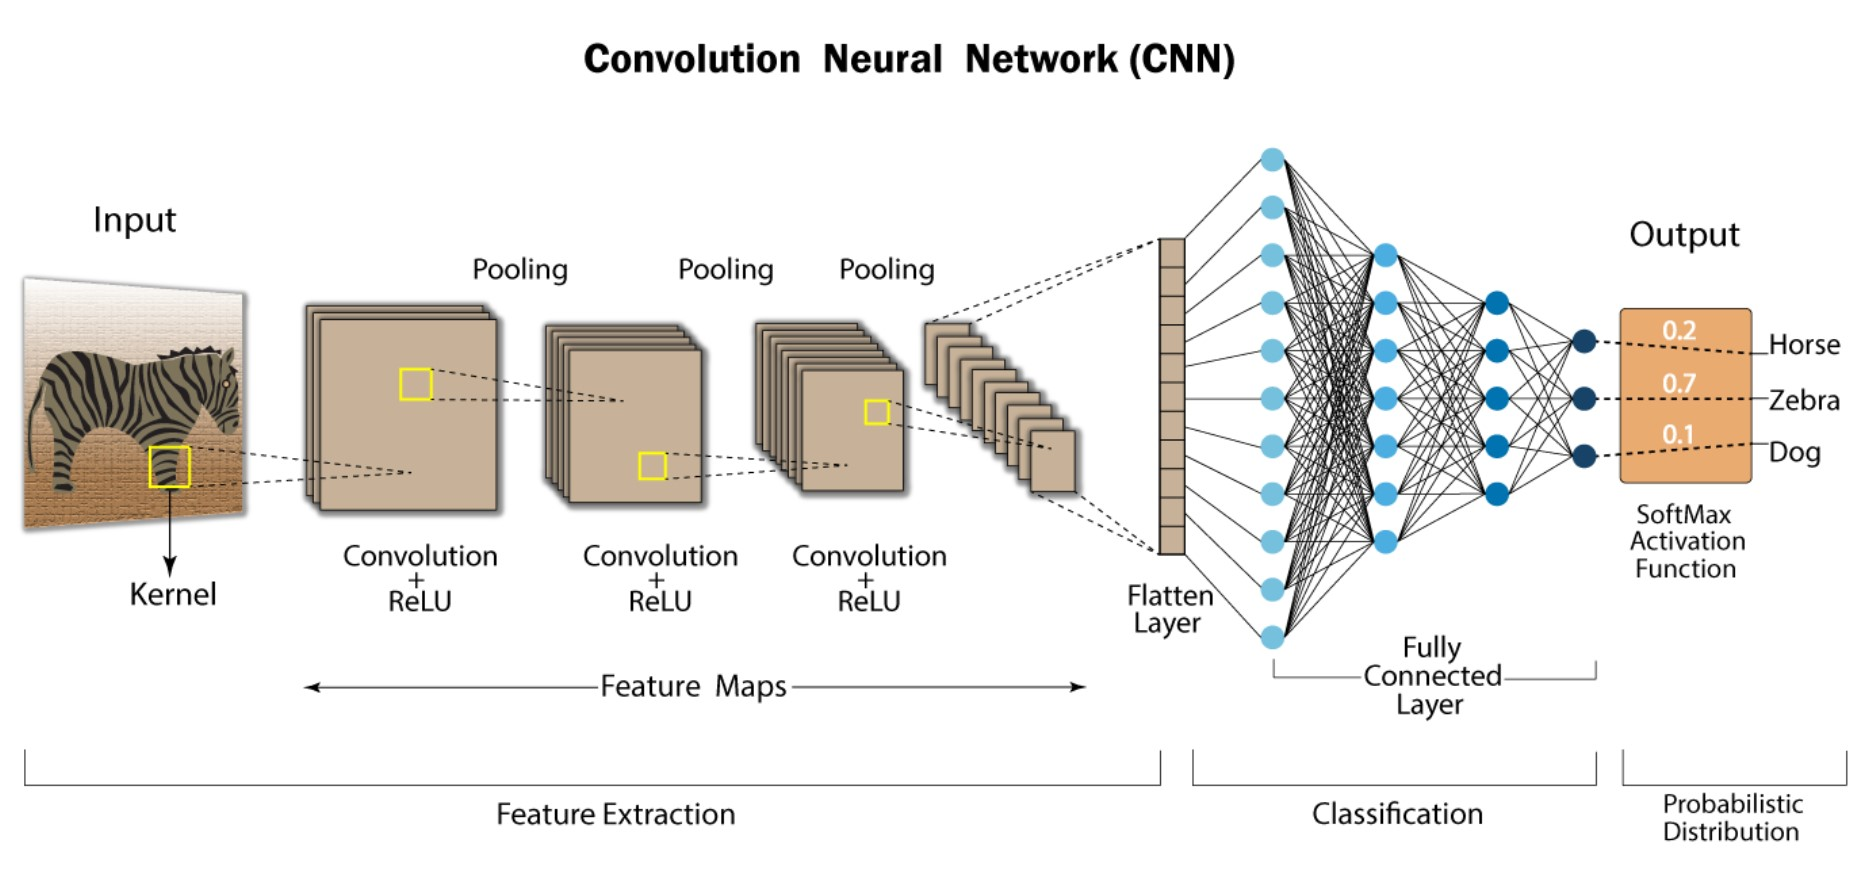
\includegraphics[width=16cm]{ESP32/cnn}
		\caption{A CNN sequence to classify handwritten digits} 
		\label{fig:A CNN sequence to classify handwritten digits}
		\footnotesize \textbf{Reference:} \cite{Swapna:2022}
	\end{center}
\end{figure}



The major part of the computation takes place at this layer. The components of the convolution layer are the input data, filters and feature map. The filter is also known as kernel or a feature detector. The feature detector moves through the recurring fields of the picture, while checking if the feature is present. This entire process is termed as convolution.

The Kernel is a two-dimensional array of biases or weights, which represents a part of the picture. The kernel can be of different sizes. This size of the kernel influences the size of receptive field. A dot product is computed between the kernel and the filter. This value of the dot product is then provided into an output array. Then the kernel moves to the next stride, this process is repeated until the kernel moves across the full picture. The final output is termed as a convolved feature or a feature map. The initial feature map only captures Low-Level information like the colour gradient and edges. The progressing feature maps captures high-level information which results in the network that helps classification of individual features present in the image. \cite{IBM:2020}

\subsection{Pooling Layer}

Pooling conducts a dimensionality reduction of the feature map. This is done by reducing the number of input parameters. Here the CNN retains the important features of the map which is required for the classification. This process is termed as down sampling.

In the pooling operation a filter without any weights is used to sweep across the whole input. Here an aggregation function is applied to the values of the receptive field by the kernel. The values of the aggregation function are used to populate the output array. \cite{IBM:2020}

\begin{itemize}
	\item \textbf{Max Pooling}:	As the kernel is swept through the input, the kernel identifies the pixel with the highest value and transfers it into the output array. This helps in retaining the most important features present in the feature map.
	\item \textbf{Average Pooling}:	As the kernel is swept through the input, it computes the average value of the receptive field and transfers it into the output array.
\end{itemize}

\begin{figure}  
	\begin{center}
		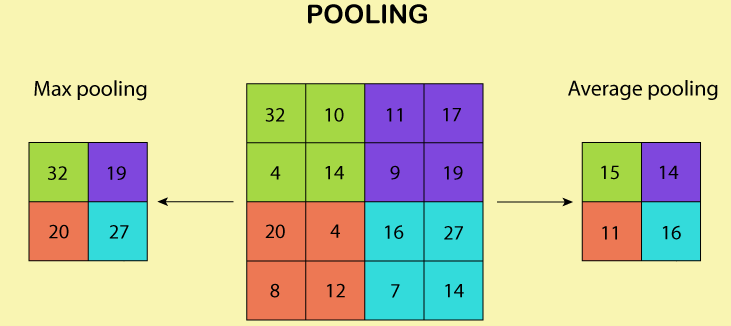
\includegraphics[width=14cm]{ESP32/PoolingLayer}
		\caption{Pooling Layer in CNN} 
		\label{Pooling Layer in CNN}
		\footnotesize \textbf{Reference:} \cite{Swapna:2022}
	\end{center}
\end{figure}

Pooling has benefits such as, limiting the risk of overfitting, size reduction, noise suppression and reduction in complexity of the feature map. These result in improved efficiency of the feature map.

\subsection{Fully-Connected Layer}

The fully-connected layer is the final layer of the CNN. Here each node of the output layer directly connects to a node of the previous layer. The classification process carried out in this layer based upon the previous layers and their appropriate filters. A Soft-Max function assigns decimal probabilities from 0 to 1 based on the appropriate classification of the inputs. \cite{IBM:2020}

\subsection{CNN Example with code}

In the following section, the required steps to train a \ac{cnn}, will be covered. There are six large sections of the code that need to be taken into account, each one of them with its own characteristics and functions. Also, the inputs and output from each code section needs to be taken into account as a priority to understand the codes functionality. 

The main sections to create and train the \ac{cnn} are the following:  

\begin{enumerate}
	\item Preparation (loading the libraries and settings).
	\item Loading the training images.
	\item Generate training data and test data.
	\item Definition and structure of the network.
	\item Train the model.
	\item Storing the neural network.
\end{enumerate}

Now with this sections clear, it is time to jump into the coding implementation. For this it is provided the following example, including comments thru out the different code lines to better understand the purpose: 

\section{Training of the CNN}


\subsection{Preparation}

\subsubsection{Libraries}

It is required to import different libraries for file and image processing, as well as for the definition
and construction of neural networks using the Tensorflow library. Therefor the first step is to load
all these libraries into the program:

\begin{code}
  \lstinputlisting[language=python,firstline=1,lastline=10,firstnumber=1]{../../Code/ESP32/CNNTraining.py}    

  \caption{Import of the packages} 
    
\end{code}    

\subsubsection{Model name}

Next it is important to define the developed model in order to distinguish between different versions
of the neural network. It is necesary to assign a unique name for the model before start running
its training or testing. This name should be identical at the beginning of each script so that the
same data is used consistently.

\medskip

\begin{code}
    \lstinputlisting[language=python,firstline=1,lastline=10,firstnumber=13]{../../Code/ESP32/CNNTraining.py}    
    
    \caption{Name of the model} 
    
\end{code}    


\subsection{Loading the training images}

For this CNN, as we stated at the beginning of this section it is required to provide an input
of images, that will be used to train and test the model. These images are loaded from a local
directory; for this matter, it is used in this directory: ``cnnModelImages'' - which can be found under
the ``CNN'' inside ``Code'' section of the GitHub Repo.

For classification purposes, this input needs to be standardized for the program to understand them.
Therefore it is also necessary for addition to the image (.jpg), that the file name is set properly and
1
according to the following nomenclature: First Character is the identifier and the rest of the name
is not relevant.
Now the output of this section will be the proper classification of the images into two arrays \PYTHON{x\_data}
(image data) and \PYTHON{y\_data} (classification):

\begin{code}
    \lstinputlisting[language=python,firstline=15,lastline=15,firstnumber=15]{../../Code/ESP32/CNNTraining.py}    
    
    \caption{} 
    
\end{code}    

\subsection{Generate training data and test data}

\subsubsection{Merge and slice the training}

Once the data set is ready to be transferred to the model it is important to implement some  functions that will allow the model to be properly fit. The first thing is to mix the loaded images,  this is done with the function shuffle. It is important in this step to make sure that both \PYTHON{x\_data} and \PYTHON{y\_data} allocation in the array is preserved since this will allow the model to distinguish the number of images.

With the data properly mixed it is time to generate the output for this section of the code, one of the key sections, for the model. The image data is going to be divided into output sets of data: 
    
\begin{itemize}
  \item  Training data (\PYTHON{x\_train} and \PYTHON{y\_train}) 
  \item  Test data (\PYTHON{x\_test} and \PYTHON{y\_test})
\end{itemize}

Important to take into account that in this case 80\% of the data will be used for training and the  remaining 20\% is going to be used exclusively for evaluation of the model performance.


\begin{code}
    \lstinputlisting[language=python,firstline=17,lastline=43,firstnumber=17]{../../Code/ESP32/CNNTraining.py}    
    
    \caption{Merge and slice the training} 
    
\end{code}    


\subsubsection{Image augmentation}

Some data transformation is required for the input images to be properly handled. For this specific action, there will not be much data, since this will be covered in the coming ‘Development’ Section of this same report. ImageDataGenerator function takes from the first definition section which random modifications to the input images will be implemented over the various parameters (shift, brightness, zoom, rotation) and then outputs them. A batch size of 4 is defined and used here, this is chosen since it has proven to be very effective when creating a network that will work with geometries. The generator is applied to both the training and test data.

\begin{code}
    \lstinputlisting[language=python,firstline=45,lastline=53,firstnumber=45]{../../Code/ESP32/CNNTraining.py}    
    
    \caption{Image augmentation} 
    
\end{code}    

\section{Definition and structure of the network}

It is now the moment to identify the specifications of the implemented network. In this case, the layout consists of a sequence of convolutional and maxpooling layers.

\begin{enumerate}
  \item The first layer is used to  normalize the input data. 
  \item The second layer is a “flat” layer with 512 neurons.
\end{enumerate}    

\subsection{Inputs}

Images of size 32x20 pixels with 3 color channels: \PYTHON{input\_shape = (32,20,3)}
  
  
\subsection{Output}

 11 neurons: Digits 0, 1,\ldots, 9 + Not-A-Number (N/A) as a special case.
 
 
\subsection{Compile}

Finally, the network is compiled here so that it can be used. The detailed parameters for this can be found in the relevant literature

\begin{code}
    \lstinputlisting[language=python,firstline=55,lastline=73,firstnumber=55]{../../Code/ESP32/CNNTraining.py}    
    
    \caption{Compile of the example} 
    
\end{code}    



\begin{verbatim}
Model: "sequential"
_________________________________________________________________
Layer (type)                              Output Shape     Param #
=================================================================
batch_normalization (BatchNormalization) (None, 32, 20, 3)  12
module_wrapper (ModuleWrapper)           (None, 32, 20, 16) 448
module_wrapper_1 (ModuleWrapper)         (None, 16, 10, 16)  0
module_wrapper_2 (ModuleWrapper)         (None, 16, 10, 32)  4640
module_wrapper_3 (ModuleWrapper)         (None, 8, 5, 32)    0
module_wrapper_4 (ModuleWrapper)         (None, 8, 5, 16)    4624
module_wrapper_5 (ModuleWrapper)         (None, 4, 2, 16)    0
module_wrapper_6 (ModuleWrapper)         (None, 128)         0
module_wrapper_7 (ModuleWrapper)         (None, 128)         16512
module_wrapper_8 (ModuleWrapper)         (None, 11)          1419
=================================================================
Total params: 27,655
Trainable params: 27,649
Non-trainable params: 6
_________________________________________________________________    
\end{verbatim}

\subsection{Training the network}

For training one of the more important concepts to take into account is the number of training cycles (\PYTHON{Epoch\_Number}). And here also comes into play the size of the simultaneously trained images, which was previously defined as 4 (\PYTHON{Batch\_Size}).

With these two factor the model will run over the total set of training data and will fit the model accordingly to best match the provided input.

\begin{code}
    \lstinputlisting[language=python,firstline=75,lastline=89,firstnumber=75]{../../Code/ESP32/CNNTraining.py}    
    
    \caption{Training the network} 
    
\end{code}    



\begin{verbatim}
Epoch 1/50
98/98 [==============================] - 3s 18ms/step - loss: 2.1443 - accuracy: 
0.4158 - val_loss: 2.0649 - val_accuracy: 0.3469
Epoch 2/50
98/98 [==============================] - 1s 13ms/step - loss: 1.9682 - accuracy: 
0.4158 - val_loss: 1.9113 - val_accuracy: 0.3571
Epoch 3/50
98/98 [==============================] - 1s 13ms/step - loss: 1.7875 - accuracy:
0.4413 - val_loss: 1.8866 - val_accuracy: 0.3673
Epoch 4/50
98/98 [==============================] - 1s 13ms/step - loss: 1.5501 - accuracy:
0.5051 - val_loss: 1.5655 - val_accuracy: 0.5000
Epoch 5/50
98/98 [==============================] - 1s 13ms/step - loss: 1.5007 - accuracy:
0.5204 - val_loss: 1.5421 - val_accuracy: 0.4796
Epoch 6/50
98/98 [==============================] - 1s 13ms/step - loss: 1.2596 - accuracy:
0.5893 - val_loss: 1.3638 - val_accuracy: 0.5102
Epoch 7/50
98/98 [==============================] - 1s 13ms/step - loss: 1.1482 - accuracy:
0.6352 - val_loss: 1.1886 - val_accuracy: 0.6327
Epoch 8/50
98/98 [==============================] - 1s 12ms/step - loss: 0.9293 - accuracy:
0.7092 - val_loss: 1.1215 - val_accuracy: 0.6429
Epoch 9/50
98/98 [==============================] - 1s 12ms/step - loss: 0.8761 - accuracy:
0.7015 - val_loss: 1.0848 - val_accuracy: 0.6633
Epoch 10/50
98/98 [==============================] - 1s 13ms/step - loss: 0.7541 - accuracy:
0.7474 - val_loss: 1.1371 - val_accuracy: 0.6633
Epoch 11/50
98/98 [==============================] - 1s 13ms/step - loss: 0.7432 - accuracy:
0.7628 - val_loss: 1.0454 - val_accuracy: 0.6633
Epoch 12/50
98/98 [==============================] - 1s 12ms/step - loss: 0.6782 - accuracy:
0.7551 - val_loss: 1.0191 - val_accuracy: 0.7143
Epoch 13/50
98/98 [==============================] - 1s 12ms/step - loss: 0.6333 - accuracy:
0.7730 - val_loss: 1.0637 - val_accuracy: 0.7143
Epoch 14/50
98/98 [==============================] - 1s 13ms/step - loss: 0.6489 - accuracy:
0.7908 - val_loss: 0.9205 - val_accuracy: 0.7041
Epoch 15/50
98/98 [==============================] - 1s 13ms/step - loss: 0.5948 - accuracy:
0.7985 - val_loss: 0.8216 - val_accuracy: 0.7245
Epoch 16/50
98/98 [==============================] - 1s 12ms/step - loss: 0.5251 - accuracy:
0.8087 - val_loss: 0.8158 - val_accuracy: 0.7551
Epoch 17/50
98/98 [==============================] - 1s 12ms/step - loss: 0.6191 - accuracy:
0.7985 - val_loss: 0.7756 - val_accuracy: 0.7347
Epoch 18/50
98/98 [==============================] - 1s 12ms/step - loss: 0.5469 - accuracy:
0.8265 - val_loss: 0.8434 - val_accuracy: 0.7143
Epoch 19/50
98/98 [==============================] - 1s 13ms/step - loss: 0.4843 - accuracy:
0.8444 - val_loss: 0.8002 - val_accuracy: 0.7755
Epoch 20/50
98/98 [==============================] - 1s 13ms/step - loss: 0.5197 - accuracy:
0.8444 - val_loss: 0.8632 - val_accuracy: 0.7041
Epoch 21/50
98/98 [==============================] - 1s 12ms/step - loss: 0.4779 - accuracy:
0.8571 - val_loss: 0.8375 - val_accuracy: 0.7449
Epoch 22/50
98/98 [==============================] - 1s 13ms/step - loss: 0.4117 - accuracy:
0.8699 - val_loss: 0.8594 - val_accuracy: 0.7653
Epoch 23/50
98/98 [==============================] - 1s 12ms/step - loss: 0.4668 - accuracy:
0.8444 - val_loss: 0.9214 - val_accuracy: 0.7143
Epoch 24/50
98/98 [==============================] - 1s 12ms/step - loss: 0.3587 - accuracy:
0.8750 - val_loss: 0.7608 - val_accuracy: 0.7857
Epoch 25/50
98/98 [==============================] - 1s 13ms/step - loss: 0.4094 - accuracy:
0.8673 - val_loss: 0.7783 - val_accuracy: 0.8061
Epoch 26/50
98/98 [==============================] - 1s 13ms/step - loss: 0.4493 - accuracy:
0.8622 - val_loss: 0.6756 - val_accuracy: 0.8163
Epoch 27/50
98/98 [==============================] - 1s 13ms/step - loss: 0.4481 - accuracy:
0.8750 - val_loss: 0.7532 - val_accuracy: 0.7857
Epoch 28/50
98/98 [==============================] - 1s 13ms/step - loss: 0.3530 - accuracy:
0.8929 - val_loss: 0.8846 - val_accuracy: 0.7143
Epoch 29/50
98/98 [==============================] - 1s 12ms/step - loss: 0.3040 - accuracy:
0.9005 - val_loss: 0.7868 - val_accuracy: 0.7653
Epoch 30/50
98/98 [==============================] - 1s 13ms/step - loss: 0.3558 - accuracy:
0.8929 - val_loss: 0.8299 - val_accuracy: 0.7755
Epoch 31/50
98/98 [==============================] - 1s 12ms/step - loss: 0.3190 - accuracy:
0.8929 - val_loss: 0.6582 - val_accuracy: 0.7959
Epoch 32/50
98/98 [==============================] - 1s 13ms/step - loss: 0.2992 - accuracy:
0.9362 - val_loss: 0.9584 - val_accuracy: 0.8163
Epoch 33/50
98/98 [==============================] - 1s 12ms/step - loss: 0.3456 - accuracy:
0.8903 - val_loss: 0.6098 - val_accuracy: 0.8265
Epoch 34/50
98/98 [==============================] - 1s 13ms/step - loss: 0.2796 - accuracy:
0.9107 - val_loss: 0.6716 - val_accuracy: 0.7755
Epoch 35/50
98/98 [==============================] - 1s 13ms/step - loss: 0.3834 - accuracy:
0.8699 - val_loss: 0.7031 - val_accuracy: 0.7857
Epoch 36/50
98/98 [==============================] - 1s 13ms/step - loss: 0.2575 - accuracy:
0.9209 - val_loss: 0.8095 - val_accuracy: 0.8163
Epoch 37/50
98/98 [==============================] - 1s 13ms/step - loss: 0.2456 - accuracy:
0.9209 - val_loss: 0.7661 - val_accuracy: 0.8061
Epoch 38/50
98/98 [==============================] - 1s 13ms/step - loss: 0.2745 - accuracy:
0.9133 - val_loss: 0.9254 - val_accuracy: 0.7755
Epoch 39/50
98/98 [==============================] - 1s 13ms/step - loss: 0.3168 - accuracy:
0.9158 - val_loss: 0.7265 - val_accuracy: 0.7959
Epoch 40/50
98/98 [==============================] - 1s 12ms/step - loss: 0.3356 - accuracy:
0.9005 - val_loss: 0.7074 - val_accuracy: 0.7959
Epoch 41/50
98/98 [==============================] - 1s 12ms/step - loss: 0.2670 - accuracy:
0.9107 - val_loss: 0.9057 - val_accuracy: 0.7653
Epoch 42/50
98/98 [==============================] - 1s 12ms/step - loss: 0.2628 - accuracy:
0.9082 - val_loss: 0.5808 - val_accuracy: 0.8265
Epoch 43/50
98/98 [==============================] - 1s 12ms/step - loss: 0.3258 - accuracy:
0.9158 - val_loss: 0.5568 - val_accuracy: 0.7959
Epoch 44/50
98/98 [==============================] - 1s 12ms/step - loss: 0.2320 - accuracy:
0.9311 - val_loss: 0.5323 - val_accuracy: 0.8265
Epoch 45/50
98/98 [==============================] - 1s 12ms/step - loss: 0.2319 - accuracy:
0.9235 - val_loss: 0.8088 - val_accuracy: 0.8163
Epoch 46/50
98/98 [==============================] - 1s 12ms/step - loss: 0.1818 - accuracy:
0.9388 - val_loss: 0.5199 - val_accuracy: 0.8571
Epoch 47/50
98/98 [==============================] - 1s 11ms/step - loss: 0.1760 - accuracy:
0.9413 - val_loss: 0.5991 - val_accuracy: 0.8367
Epoch 48/50
98/98 [==============================] - 1s 12ms/step - loss: 0.1834 - accuracy:
0.9464 - val_loss: 0.7558 - val_accuracy: 0.8061
Epoch 49/50
98/98 [==============================] - 1s 12ms/step - loss: 0.1781 - accuracy:
0.9388 - val_loss: 0.7252 - val_accuracy: 0.8367
Epoch 50/50
98/98 [==============================] - 1s 12ms/step - loss: 0.2461 - accuracy:
0.9286 - val_loss: 0.7511 - val_accuracy: 0.8367
\end{verbatim}

\subsection{Visualization of training}

The model is now ready to use. For a better understanding of the output, one can be visualized how the training was performed. For this matter, the error is used, both in the training data as well as in the test data.


\begin{figure}  
    \begin{center}
        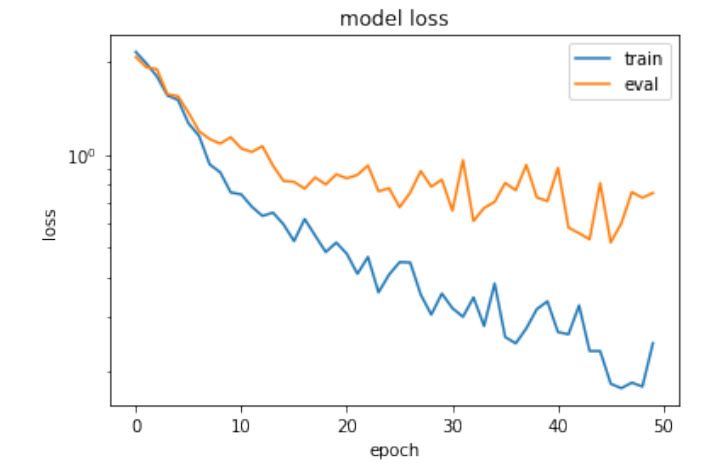
\includegraphics[width=12cm]{ESP32/CNNTraining}
        \caption{Loss functions of the training} 
        \label{ESP32fig:Lossfunctions}
    \end{center}
\end{figure}


\subsection{Saving the Neural Network}

Last step is to get the outputed neural network saved for further use. The complete network is first  saved here in the format H5.


\begin{code}
    \lstinputlisting[language=python,firstline=92,firstnumber=92]{../../Code/ESP32/CNNTraining.py}    
    
    \caption{Visualization of training} 
    
\end{code}    



\begin{verbatim}
WARNING:absl:Found untraced functions such as
conv2d_layer_call_and_return_conditional_losses, conv2d_layer_call_fn,
conv2d_1_layer_call_and_return_conditional_losses, conv2d_1_layer_call_fn,
conv2d_2_layer_call_and_return_conditional_losses while saving (showing 5 of
12). These functions will not be directly callable after loading.
INFO:tensorflow:Assets written to: saved_model/counter_det\assets
INFO:tensorflow:Assets written to: saved_model/counter_det\assets
\end{verbatim}



%%%%%%%%%%%%%%%%%%%%%%%%%%%%%%%



